%!TEX program = xelatex

\documentclass{article}
\usepackage{graphicx}

% load package with some of the available options - you may not need this!
\usepackage[framed,numbered,autolinebreaks,useliterate]{mcode}

% something NOT relevant to the usage of the package.
\usepackage{url,textcomp}
\setlength{\parindent}{0pt}
\setlength{\parskip}{18pt}
\title{\texttt{Problem1} Report}
\author{Fanyong Xue, \texttt{515030910443}}
% //////////////////////////////////////////////////

\begin{document}

\maketitle

\begin{center}
\begin{minipage}{.75\linewidth}
	\color{red}{\hfill\textbf{NOTE --- BEFORE YOU START}\hfill\strut}

	All that this package does is to configure the \verb|listings| package for you. If anything is not working the way you want it, refer to the \verb|listings| documentation first and / or take a look at the \verb|mcode.sty| file itself, which is well documented internally.\\
	
	The \verb|listings| documentation can be accessed either by typing \verb|texdoc listings| into a command prompt on your system, or online:\\\scriptsize\url{http://mirrors.ctan.org/macros/latex/contrib/listings/listings.pdf}
	
\end{minipage}
\end{center}

\section*{Installation of the package}

As with any other small package, just place the \verb|mcode.sty| file in the same folder as your document, or put it somewhere where \LaTeX{} can find it.  Done!

\medskip

\section*{Code \& Results}

1) Codes

\begin{lstlisting}
%Problem 1
%by Xue Fanyong
%Student ID:515030910443
%Histogram Equalizatio

%%main part
image1 = imread('/image path/Fig1.jpg');
image2 = imread('/image path/Fig2.jpg');

[histogram1,histogram_e1,transfer_f1,image_e1] = histogram_equalization(image1);
[histogram2,histogram_e2,transfer_f2,image_e2] = histogram_equalization(image2);

plot_data(image1,image_e1,histogram1,histogram_e1,transfer_f1);
plot_data(image2,image_e2,histogram2,histogram_e2,transfer_f2);

%%functions part

% get histogram of image
% image: get histogram of it
% histogram: the histogram of image
function histogram = get_histogram(image)
    histogram = zeros(256,1);
    [row,col]=size(image);
    for r = 1:row
        for c = 1:col
            gray = image(r,c);
            histogram(gray+1)=histogram(gray+1)+1;
        end
    end
end

%do the histogram_equalization for image
%image: do the histogram_equalization for it
%histogram: original histogram; histogram_e: histogram after histogram
%equalizatio; transfer_f: transfer function; image_e: image after histogram
%equalizatio
function [histogram,histogram_e,transfer_f,image_e] = histogram_equalization(image)
    [row,col]=size(image);
    transfer_f = zeros(256,1);
    histogram = get_histogram(image);
    transfer_f(1) = 256*histogram(1)/(row*col);
    
    for i = 2:256
        transfer_f(i) = transfer_f(i-1)+255*histogram(i)/(row*col);
    end
    transfer_f = round(transfer_f);
    
    image_e = image;
    for r = 1:row
        for c = 1:col
            image_e(r,c)=transfer_f(image(r,c)+1);
        end
    end
    histogram_e = get_histogram(image_e);
end

%plot data
%image:original image; image_e: image after histogram equalizatio; histogram: original histogram; 
%histogram_e: histogram after histogram equalizatio; transfer_f: transfer function
function plot_data(image,image_e,histogram,histogram_e,transfer_f)
    figure();
    subplot(2,3,1);
    imshow(image);
    title("Original Image");
    subplot(2,3,2);
    imshow(image_e);
    title("Image(Histogram Equalization)");
    subplot(2,3,3);
    bar(histogram);
    title("Histogram");
    subplot(2,3,4);
    bar(histogram_e);
    title("Histogram(Equalization)");
    subplot(2,3,5);
    plot(transfer_f);
    title("Transfer Funciton");
end

\end{lstlisting}

2)Results
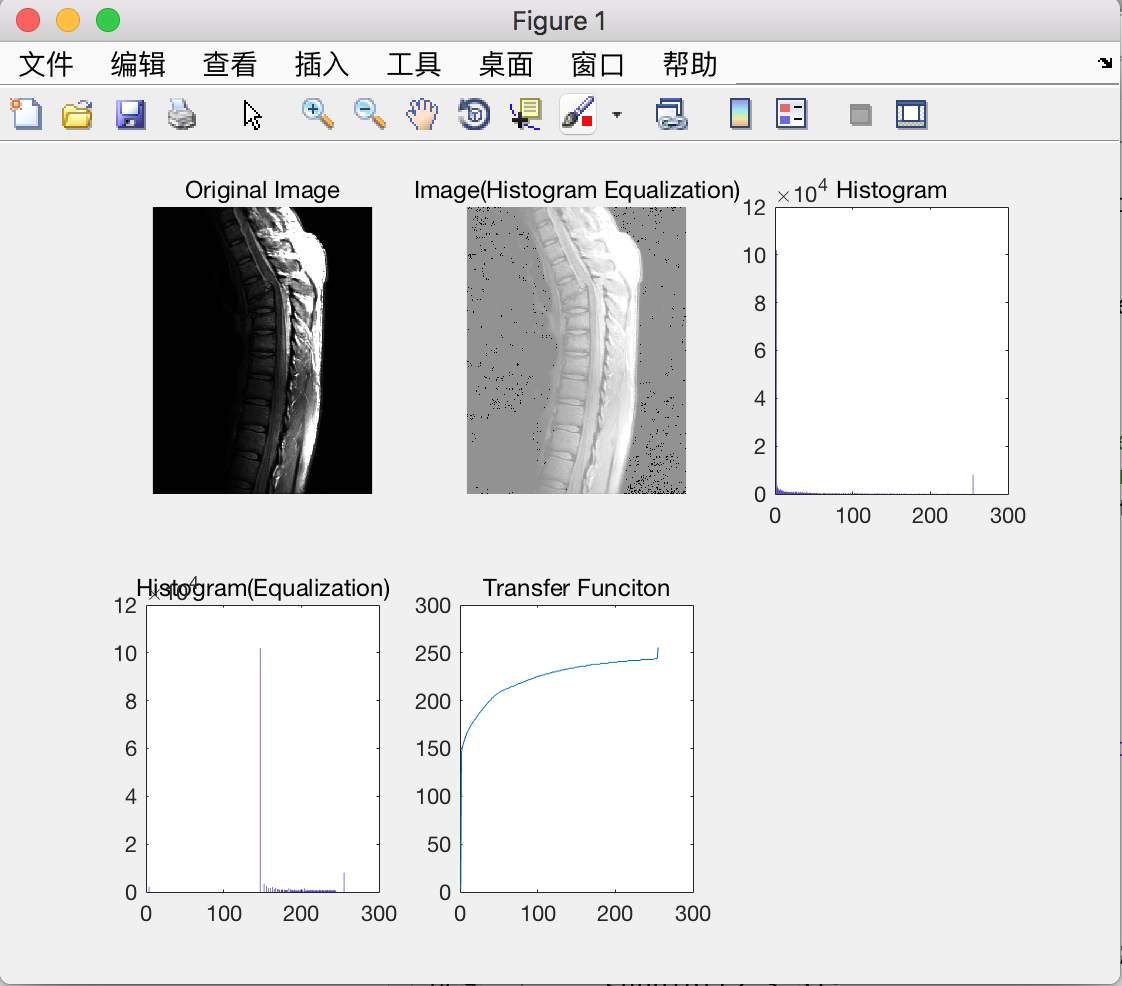
\includegraphics{/Users/xuefanyong/Documents/GitHub/DIP/Reports/report1/images/result1} 
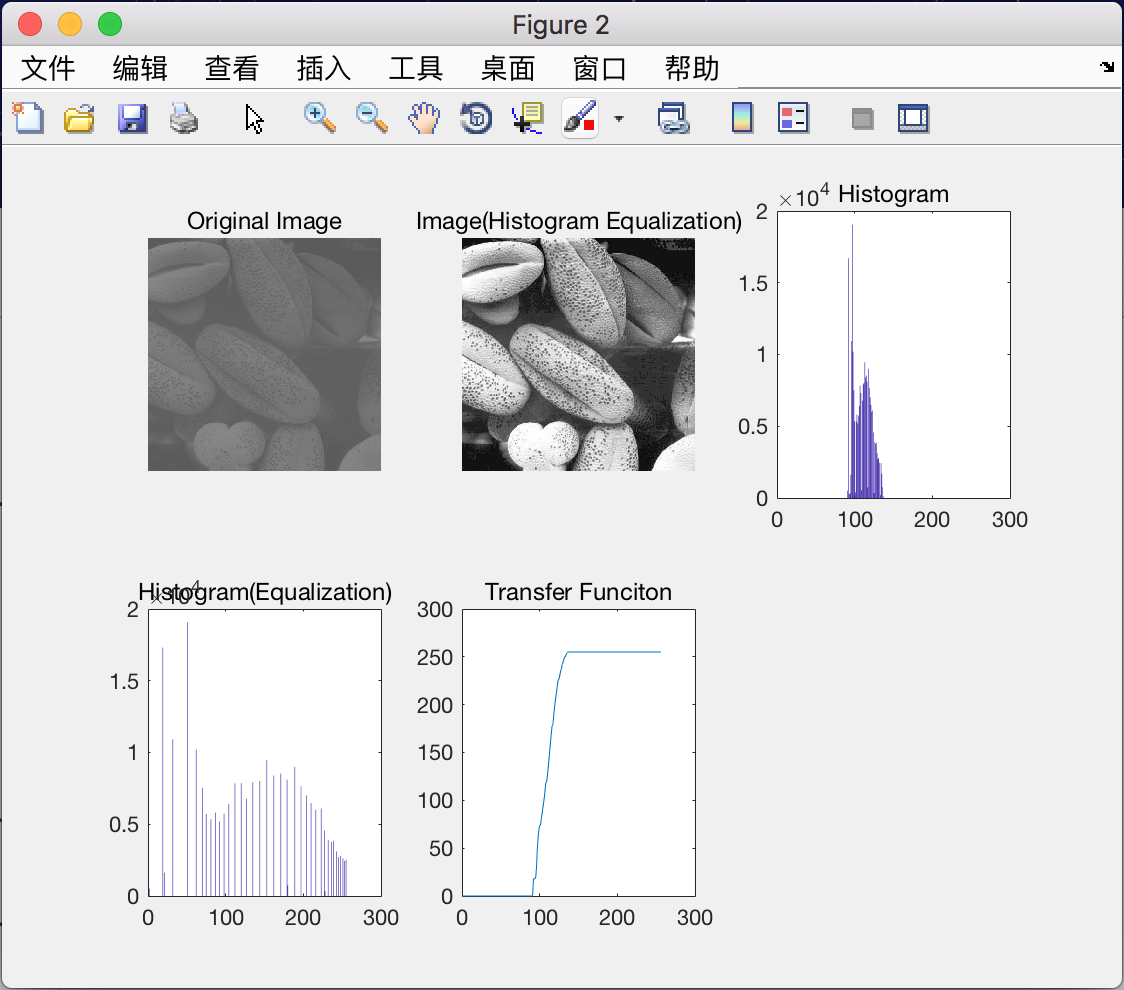
\includegraphics{/Users/xuefanyong/Documents/GitHub/DIP/Reports/report1/images/result2}



Note: Here, the package was loaded with the \verb|framed|, \verb|numbered|, \verb|autolinebreaks| and \verb|useliterate| options.  \textbf{Please see the top of mcode.sty for a detailed explanation of these options.}


3) Finally, you can also directly include an external m-file from somewhere on your hard drive (the very code you use in \textsc{Matlab}, if you want) using the \verb|\lstinputlisting{/SOME/PATH/FILENAME.M}| command.  If you only want to include certain lines from that file (for instance to skip a header), you can use \verb|\lstinputlisting[firstline=6, lastline=15]{/SOME/PATH/FILENAME.M}|.

\section*{FAQ}

\begin{description}
	\item[Why does {\tt delta} get replaced by $\Delta$, {\fontfamily{ptm}\selectfont\texttildelow=} by $\neq$, etc.?]
		Well, that's precisely what the \verb|useliterate| option does. If you don't want that, don't use it.
	\item[Can I get contiguous line numbers from one code block to another?]
		Yes, but you have to read the \verb|listings| documentation for that (Section~4.8 in particular).
	\item[{\tt mcode.sty} doesn't work in my document!] Well, try your (Matlab) code fragment in this demo document here to see whether there's something in it that might be causing a problem (not so likely, but possible), or if there's some conflict between the \verb|listings| package and some other package you have loaded.
	\item[Is feature XYZ possible?] Well, the \verb|listings| package might already be able to do that. Please consult its documentation (see red box at the top)!
\end{description}


\end{document}